\chapter{Project Architecture and Design}

In the following text, the author will describe the architecture and design of the Thesis Management System including functional and non-functional requirements of the client.

\section{Functional Requirements}

\begin{enumerate}
    \item User management\\
    The system allows to CRUD users. A user contains fields full name, email and password.

    \item Registration\\
    An anonymous user can sign up.

    \item Log In\\
    An anonymous user can sign in using email and password.

    \item Thesis topic management\\
    The system allows to create, read, update and delete (CRUD) a thesis topic. A topic contains fields title and description in two languages.

    \item Category management\\
    The system allows to CRUD categories. A category contains fields title and description.

    \item Thesis topic can be added to categories.\\
    Topics can be added to one or more categories which allows a user to browse topics in a category.

    \item Tags can be assigned to a thesis topic\\
    There can be zero or more tags assigned to a thesis topic.

    \item Thesis topic contains field for an external supervisor (owner)\\
    The supervisor has the authority to manage thesis topics created by them.

    \item University management\\
    The system allows to CRUD universities. A university contain a field for the name of the university.

    \item Thesis topic contains field for list of universities\\
    This field contains the list of universities that the topic is offered to. A thesis topic can be offered to one or more universities.

    \item Thesis topic contains field for list of supervisors\\
    This field contains the list of university supervisors, each supervisor is assigned a university that they supervise at. A thesis topic can have zero or more university supervisors.

    \item Thesis topic contains field for list of types\\
    This field contains the list of types (i.e. diploma, bachelor). A thesis topic can have zero or more types.

    \item Application management\\
    The system allows to CRUD applications.

    \item Students can apply for a thesis topic\\
    The applicant chooses the type and the university that they apply to.

    \item Application can be approved

    \item Thesis topic can be enabled or disabled

    \item Thesis topics can be filtered\\
    The system allows to filter thesis topics by university, type, owner or title.

    \item Thesis management\\
    The system allows to CRUD theses. A thesis contains fields title, description, thesis topic, assignee, supervisor, abstract, type and university.

    \item Tags can be assigned to a thesis\\
    There can be zero or more tags assigned to a topic.

    \item Thesis contains field status\\
    Status can be either `in progress', `finished', `failed' or `postponed'.

    \item Thesis contains field grade\\
    One of A, B, C, D, E or F.

    \item Supervisor can select universities they supervise at for each thesis topic

    \item Authenticated user can subscribe for a thesis topic or a thesis\\
    The system sends notifications to all subscribers of a thesis topic or a thesis when a change is made to it.

    \item Authenticated user can unsubscribe from a thesis topic or a thesis

    \item Theses can be filtered\\
    The system allows to filter theses by title, supervisor, assignee, status, grade, type or university.

    \item Theses and thesis topics can be filtered by tags\\
    The system allows to list theses or thesis topics that contains a particular tag.

    \item File management for theses\\
    The system allows to upload files to a thesis.

    \item Discussion for thesis topics and theses\\
    A logged in user can comment on thesis topics and theses.

    \item Private comments\\
    Comments that are not visible to students can be created.

    \item Full text search\\
    Theses and thesis topics can be searched by a full text search engine.

    \item Frequently Asked Questions (FAQ) management\\
    The system allows to CRUD Frequently Asked Questions. One frequently asked question contains fields question, answer and locale.

\end{enumerate}

\newpage

\subsection{Use Case Diagram}

\begin{figure}[H]
    \centering
        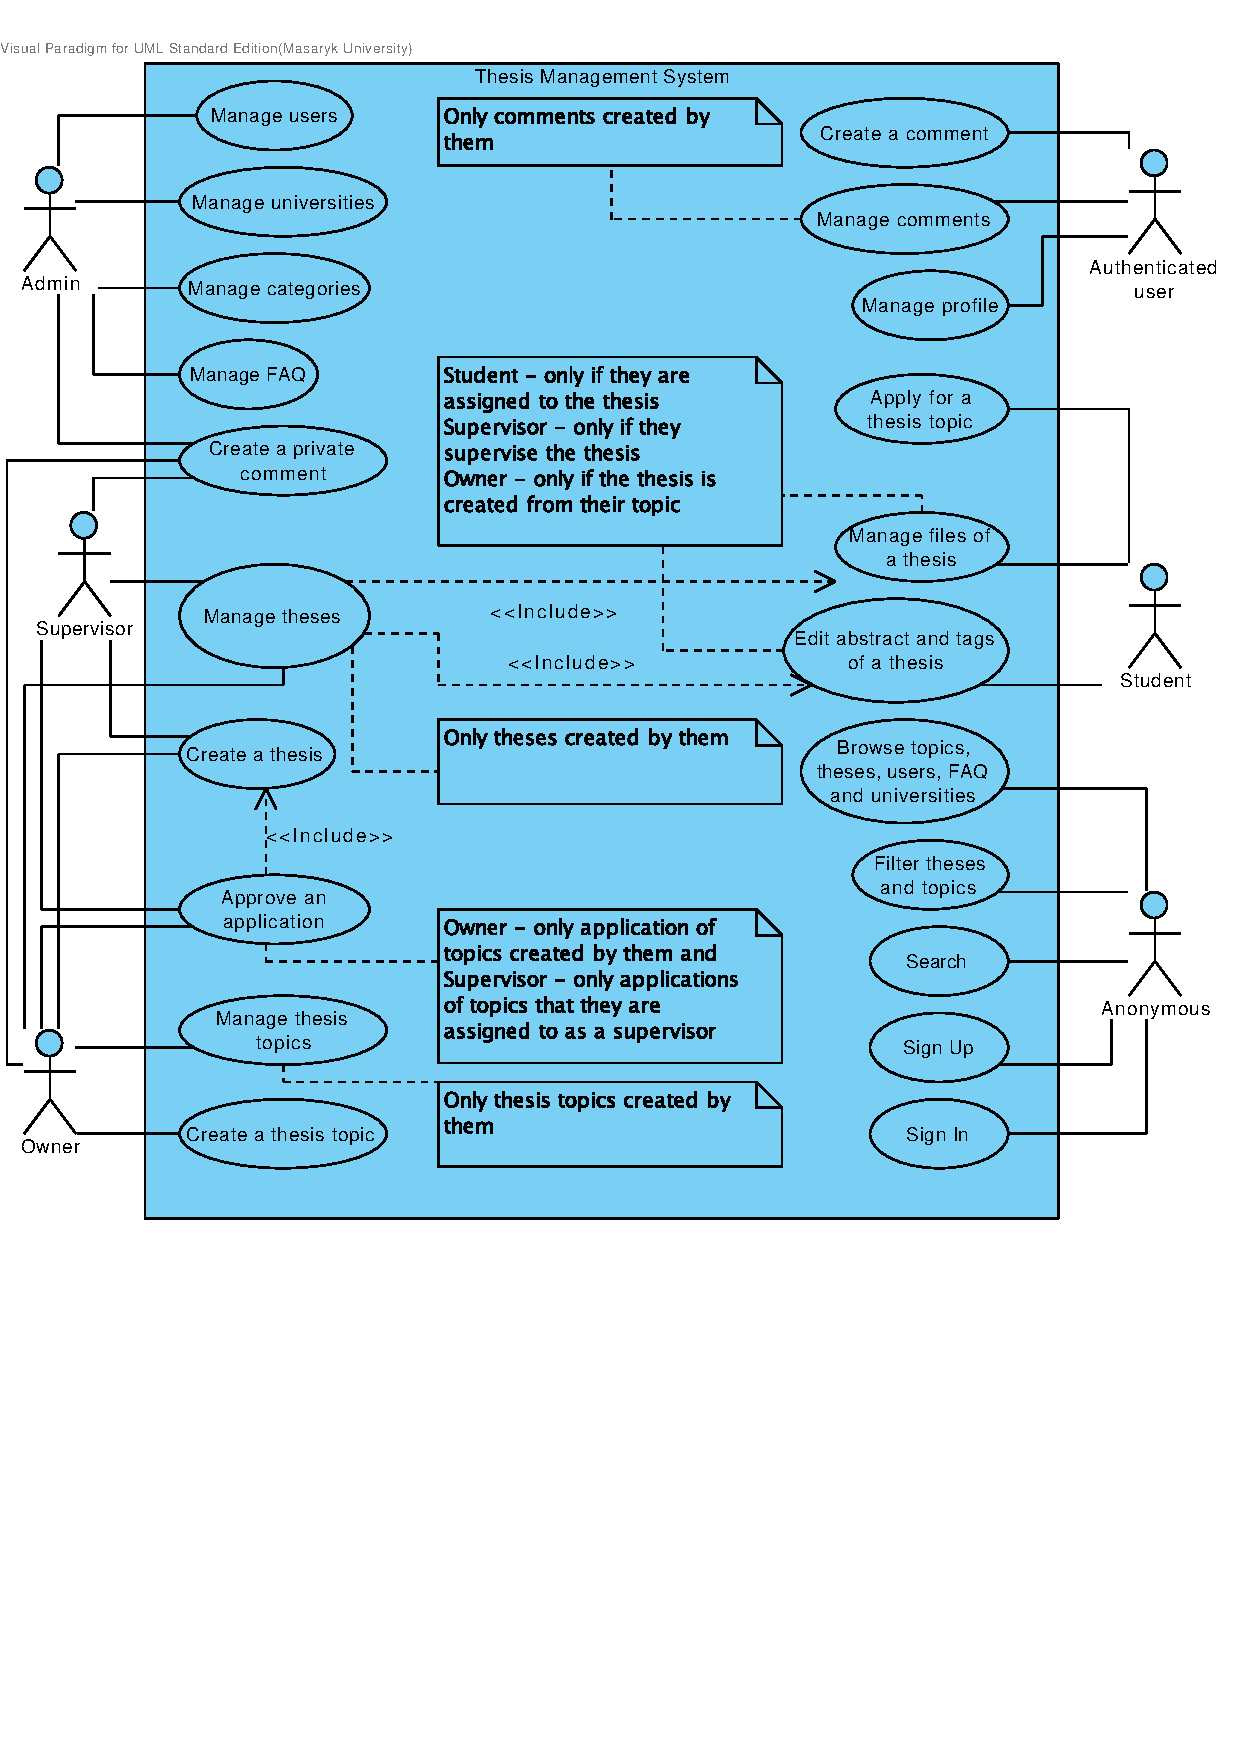
\includegraphics[trim=0 190 10 30, clip, keepaspectratio, width=\textwidth]{./images/use-case.pdf}
    \caption{Use case diagram of the Thesis Management System}
    \label{fig:use-case}
\end{figure}

\section{Non-Functional Requirements}

\begin{enumerate}
    \item Grails platform\\
    The system is implemented using platform Grails.

    \item Authentication and authorization\\
    The system is secured and there are four roles -- \textbf{Administrator} that can manage users, categories, FAQ and universities, \textbf{Owner} that can create thesis topics and manage thesis topics created by them, \textbf{Supervisor} that can create theses and manage theses created by them and \textbf{Student} that can apply for a thesis topic.

    \item Performance\\
    The system offers reasonable performance at least up to five hundred created thesis topics, theses, users and universities.

    \item Deployment\\
    The system is deployed on OpenShift using any cartridge other than Do It Yourself.

    \item License\\
    The system is licensed under any GPL compatible license.

    \item Backup\\
    Create a shell script for backing up the database.

    \item Internationalization and localization\\
    The system is internationalized and localized in English and Czech.

    \item Software development methodology\\
    The system is developed iteratively and incrementally.

\end{enumerate}

\section{Domain Model}

Designing the domain model is the most important step when designing an information system. It is also the most difficult one, because you usually cannot easily make changes in the domain model after you implemented the application logic around it. You can, however, add some domain model elements that the already-designed elements do not relate to. For example, if you design an entity \texttt{User}, you can implement it and easily add new entity \texttt{Group} later on if the \texttt{Group} is the owner of the relationship, see fig. \ref{fig:user-group-owner-example}. If the \texttt{User} is the owner of the relationship (see fig. \ref{fig:user-owner-group-example}), more refactoring is required to implement such changes (especially in case of object composition), because the fundamental API of the implemented part of the system changed.

\begin{figure}[h]
    \centering
        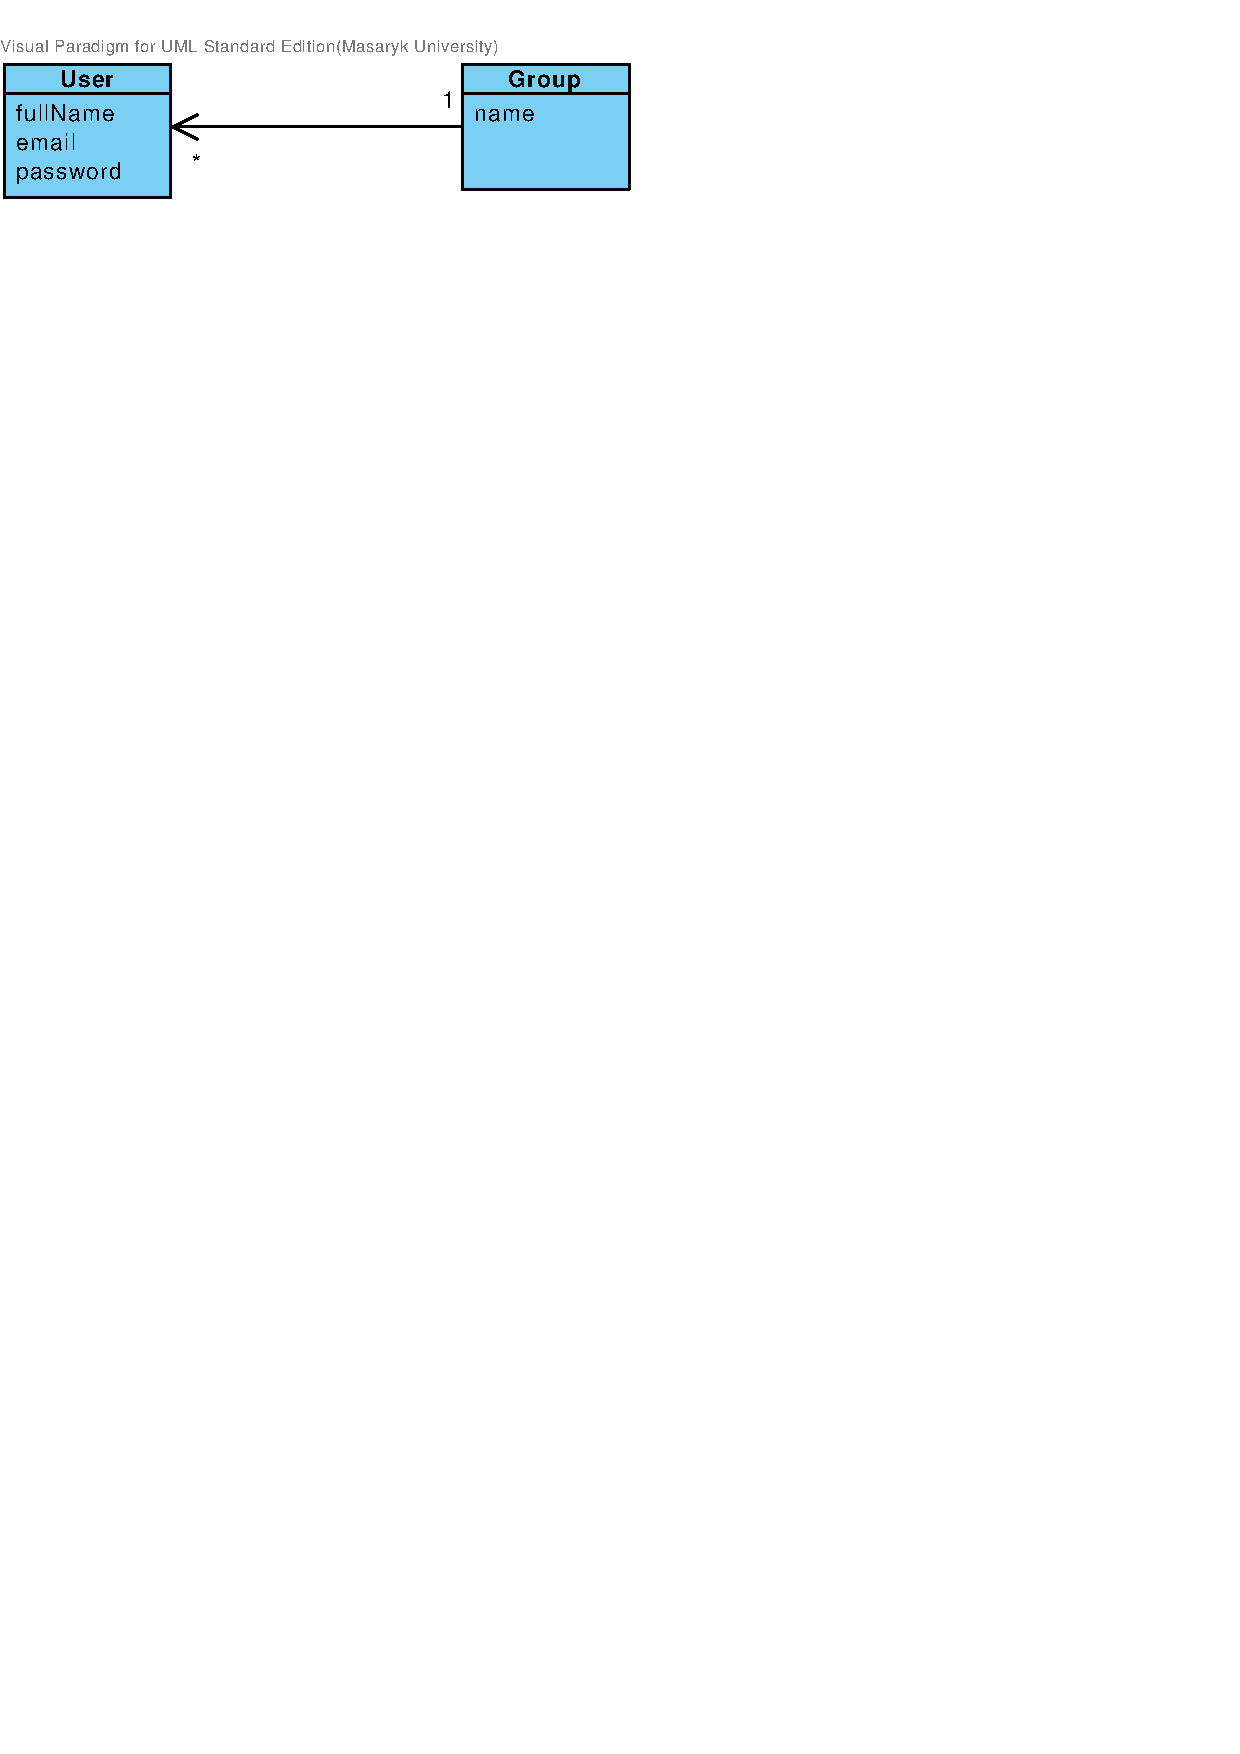
\includegraphics[trim=0 740 290 30, clip, keepaspectratio]{./images/user-group-owner-example.pdf}
    \caption{Example of domain model where \texttt{Group} owns the relationship}
    \label{fig:user-group-owner-example}
\end{figure}

\begin{figure}[h]
    \centering
        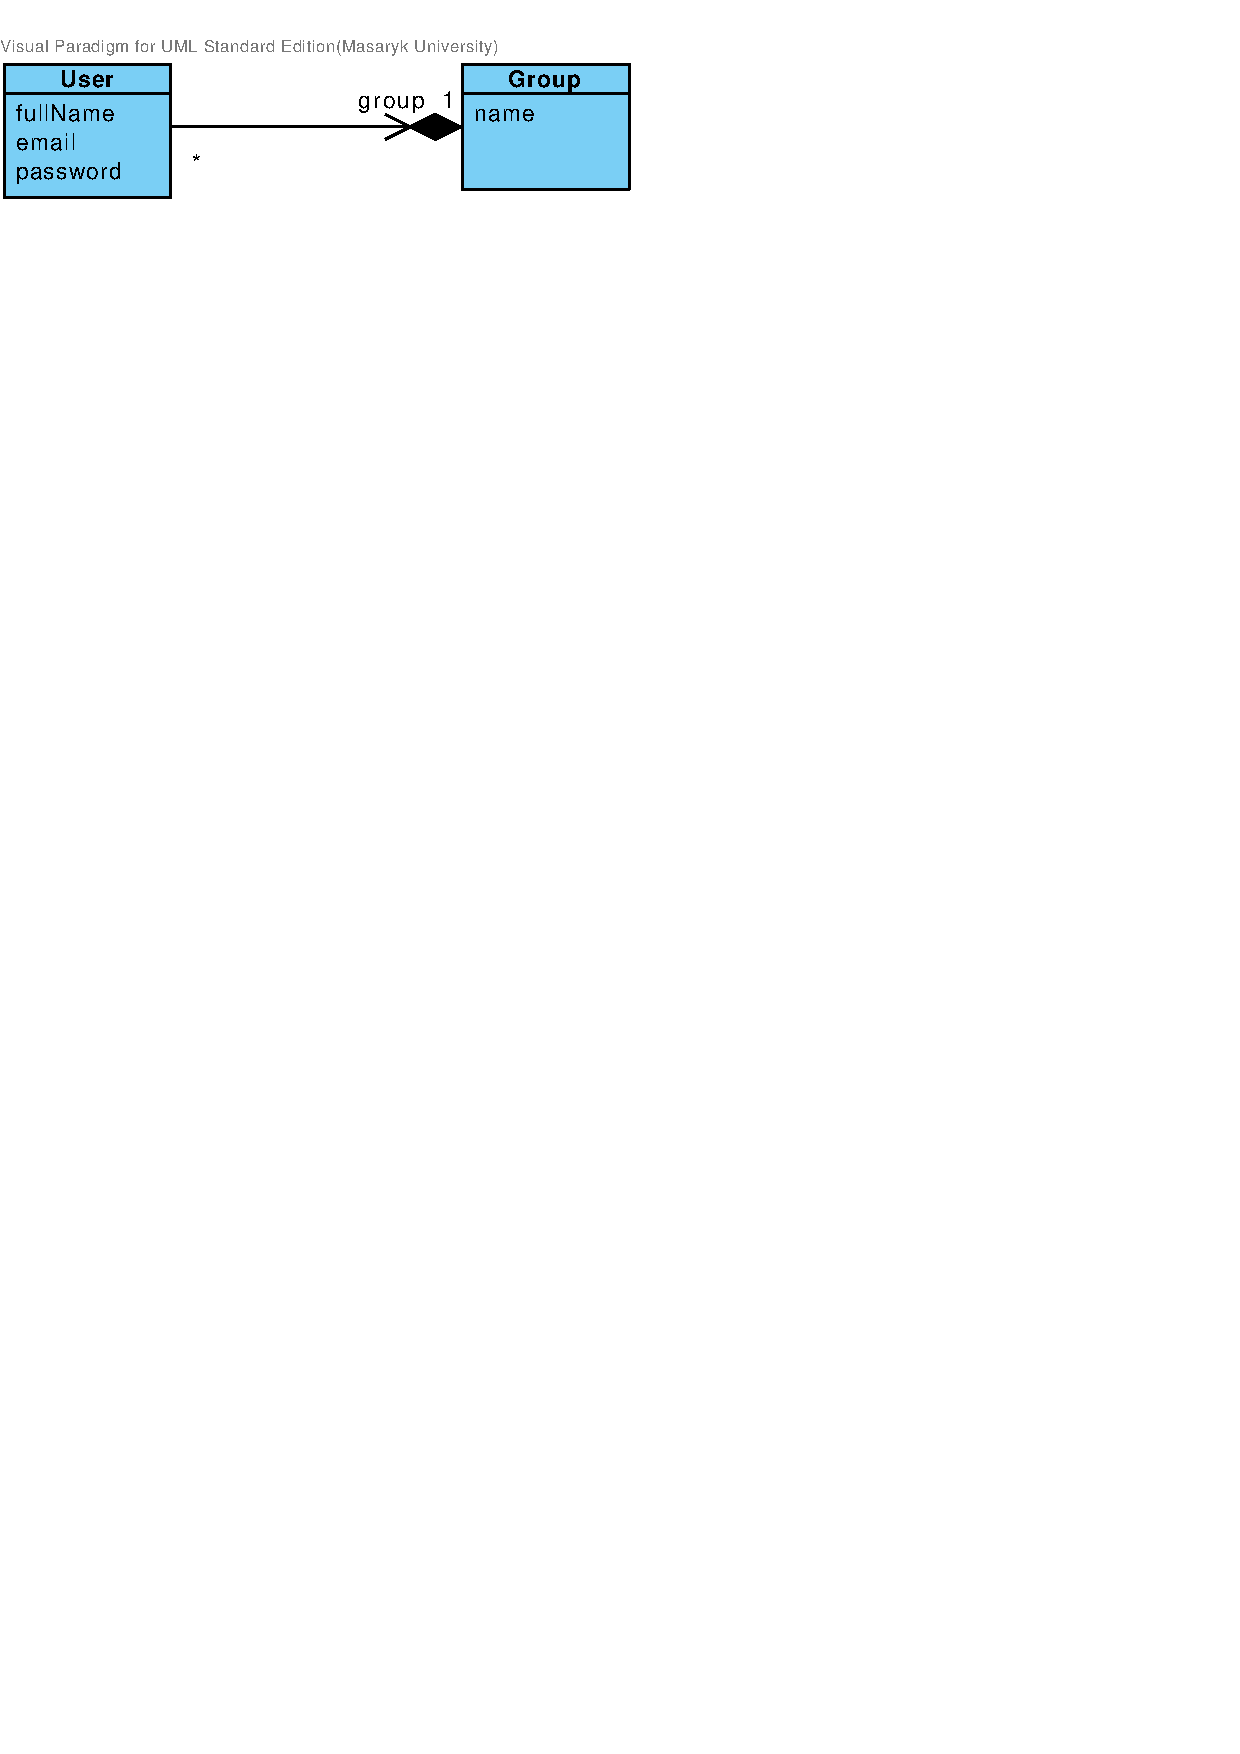
\includegraphics[trim=0 740 290 30, clip, keepaspectratio]{./images/user-owner-group-example.pdf}
    \caption{Example of domain model where \texttt{User} owns the relationship and composition is introduced}
    \label{fig:user-owner-group-example}
\end{figure}

Even more difficult can be deleting or editing attributes of an implemented entity. As a lot of refactoring is necessary to cope with such changes, a lot of new bugs is usually introduced, so it is best to avoid such changes by designing the domain model thoroughly.

Note that it is necessary to change the domain model if you implement your application incrementally. You should, however, try to minimize changes that require the API of the implemented domain model to be changed.

\subsection{Domain Model of the Thesis Management System}

As the domain model of the Thesis Management System is very complex, the author will describe it part by part.

\subsubsection{\texttt{User} entity}

To fulfill the first three functional requirements, we need to register users. For that reason, we introduce entity \texttt{User} with fields \texttt{email} and \texttt{password} that serve as log in credentials and field \texttt{fullName}. We also need fields \texttt{accountLocked} to allow the administrator to lock a user account and \texttt{enabled} for registration confirmation purposes. Field \texttt{sendMail} represents user setting that allows them to disable receiving notifications by email and field \texttt{dateCreated} represents the date of registration. To implement authorization, the \texttt{User} entity needs field \texttt{roles} which contains list of user's authorities. An authority is represented by enumeration \texttt{Role}. Figure \ref{fig:domain-user-entity} illustrates the described model.

\begin{figure}[h]
    \centering
        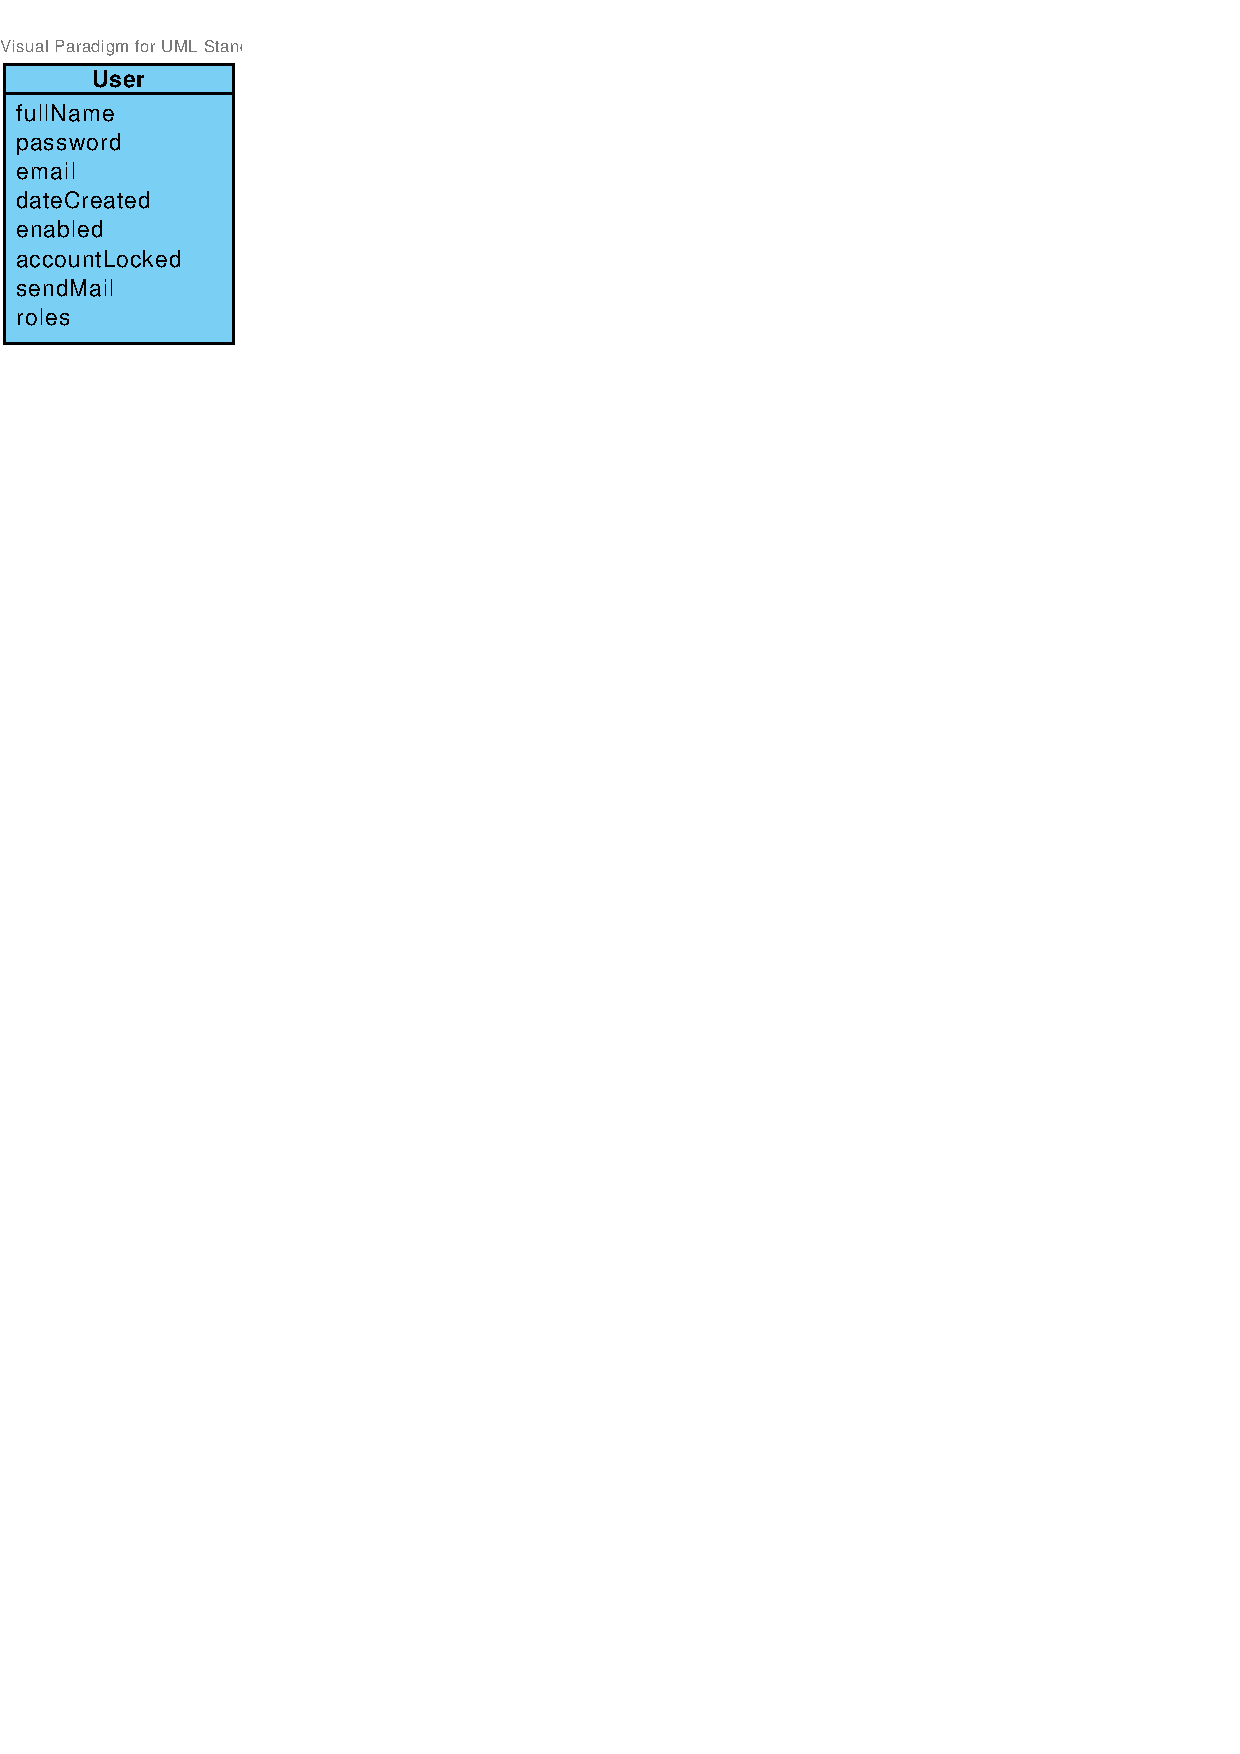
\includegraphics[trim=0 675 250 30, clip, keepaspectratio]{./images/domain-user-entity.pdf}
    \caption{\texttt{User} entity model}
    \label{fig:domain-user-entity}
\end{figure}

\subsubsection{\texttt{University} entity}

\faketext[24]